\documentclass[../midgard.tex]{subfiles}
\graphicspath{{\subfix{../images/}}}
\begin{document}

\def\txDiagramScale{0.9}

\chapter{Midgard L1 transactions}
\label{h:midgard-l1-tx}

This chapter specifies the L1 transactions that interact with Midgard's consensus protocol smart contracts.
Whereas the onchain smart contract are specified in a modular way, where each validator is only concerned with its own validity conditions, the transactions specified in this chapter often interact with several of the onchain validators and must satisfy all of their conditions.
Thus, the offchain code can be seen as the integration layer for the onchain code.

\begin{figure}[htb]
\begin{center}
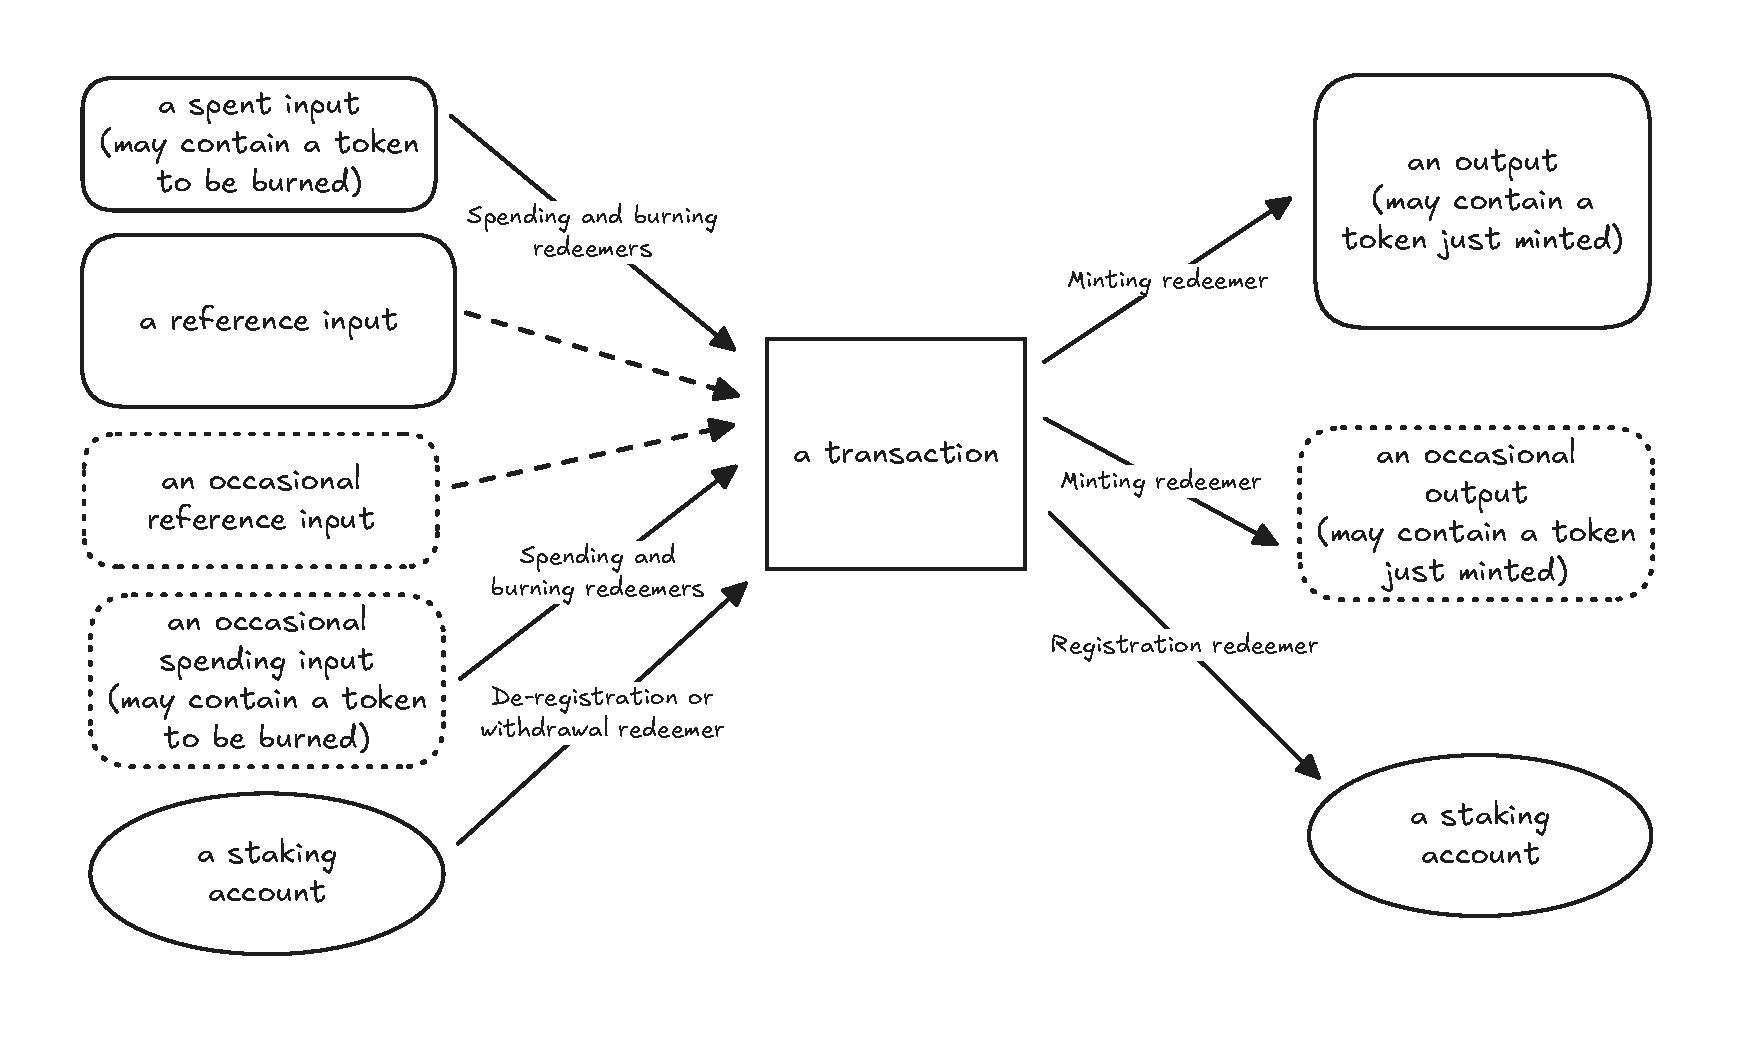
\includegraphics[width=\txDiagramScale\linewidth]{\subfix{../images/tx-diagram/Z-example-diagram.pdf}}
\end{center}
\caption[Example transaction diagram]{Example transaction diagram.}
\label{fig:tx-example}
\end{figure}

As illustrated in the example diagram (\cref{fig:tx-example}), interpret our transaction diagrams as follows:
\begin{itemize}
  \item Transactions are sharp-corner rectangles.
  \item Spent inputs are rounded-corner rectangles with outgoing arrows to transactions.
  \item Reference inputs are rounded-corner rectangles with dashed outgoing arrows to transactions.
  \item Outputs are rounded-corner rectangles with incoming arrows from transactions.
  \item Staking account are ellipses with incoming arrows from transactions if they're being registered and outgoing arrows to transactions if they're being de-registered or withdrawn from.
  \item Occasional inputs/outputs are rounded-corner rectangles with dotted borders. This indicates that these inputs/outputs may sometimes be present in transactions, but may be absent in other times.
  \item Spending redeemers label arrows from inputs to transactions.
  \item Burning redeemers label arrows from inputs to transactions, when those inputs contain tokens to be burned by the transactions.
  \item Minting redeemers label arrows from transactions to outputs, when those outputs contain tokens minted by the transactions.
  \item Redeemer labels may be omitted when scripts have only one possible redeemer.
\end{itemize}

\section{Initialization}%
\label{h:midgard-l1-tx-initialization}%

\begin{figure}[htb]
\begin{center}
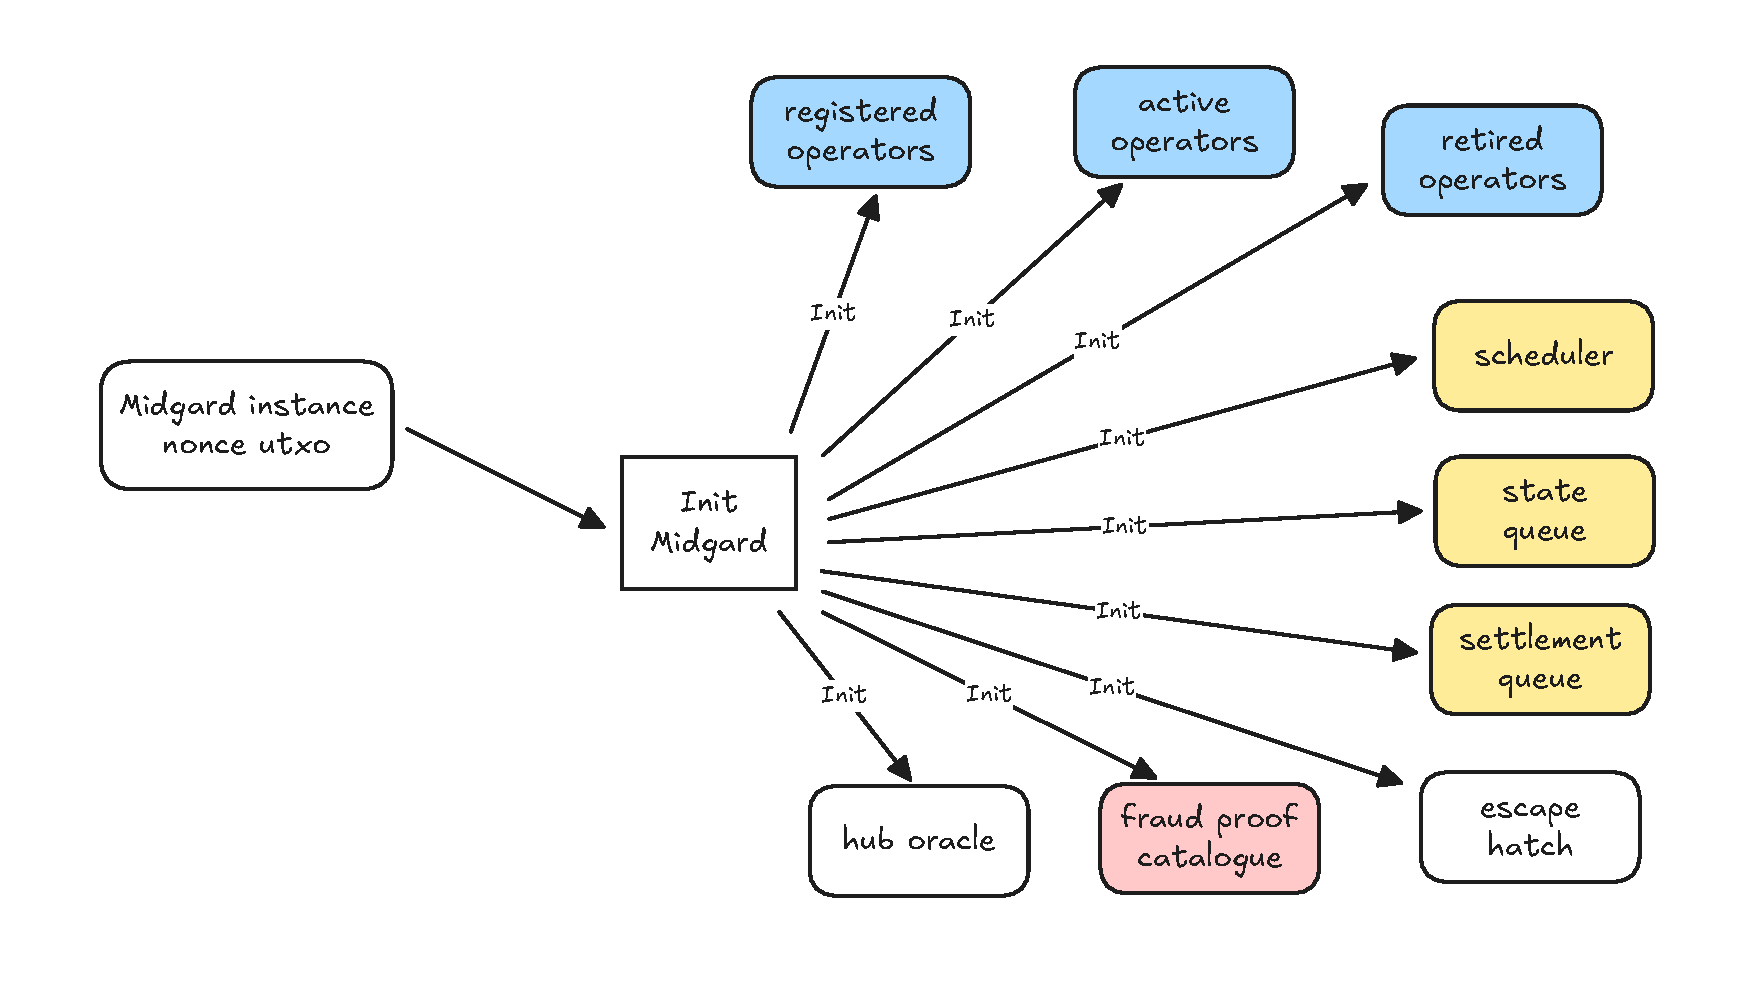
\includegraphics[width=\txDiagramScale\linewidth]{\subfix{../images/tx-diagram/0-init-midgard.pdf}}
\end{center}
\caption[Initialize Midgard]{Initialize Midgard.}
\label{fig:tx-init-midgard}
\end{figure}

A Midgard instance is initialized with a single transaction that all the onchain data structures required for Midgard's smart-contract-based consensus protocol.
This transaction:
\begin{enumerate}
  \item Spends a nonce utxo to uniquely parametrize%
    \footnote{A Midgard instance's hub oracle minting policy is parametrized on the nonce utxo spent in the initialization transaction, and all minting policies of the Midgard instance are parametrized on the hub oracle minting policy.}
    and authorize the initialization%
    \footnote{For example, if the nonce utxo is spent from a native script address, then initializing a Midgard instance parametrized by that nonce utxo must satisfy the signature and timing requirements of the native script.}
    of the Midgard instance.
  \item Produces the root nodes of the initially empty registered, active, and retired operator lists.
  \item Produces the root nodes of the initially empty state and settlement queues.
  \item Produces the scheduler, escape hatch, fraud proof catalogue, and hub oracle singleton utxos.
\end{enumerate}

The hub oracle minting policy's Init redeemer enforces the initialization transaction's correctness (see \cref{h:hub-oracle-minting-policy}).

\section{Operator management}%
\label{h:midgard-l1-tx-operator-management}%

\begin{figure}[htb]
\begin{center}
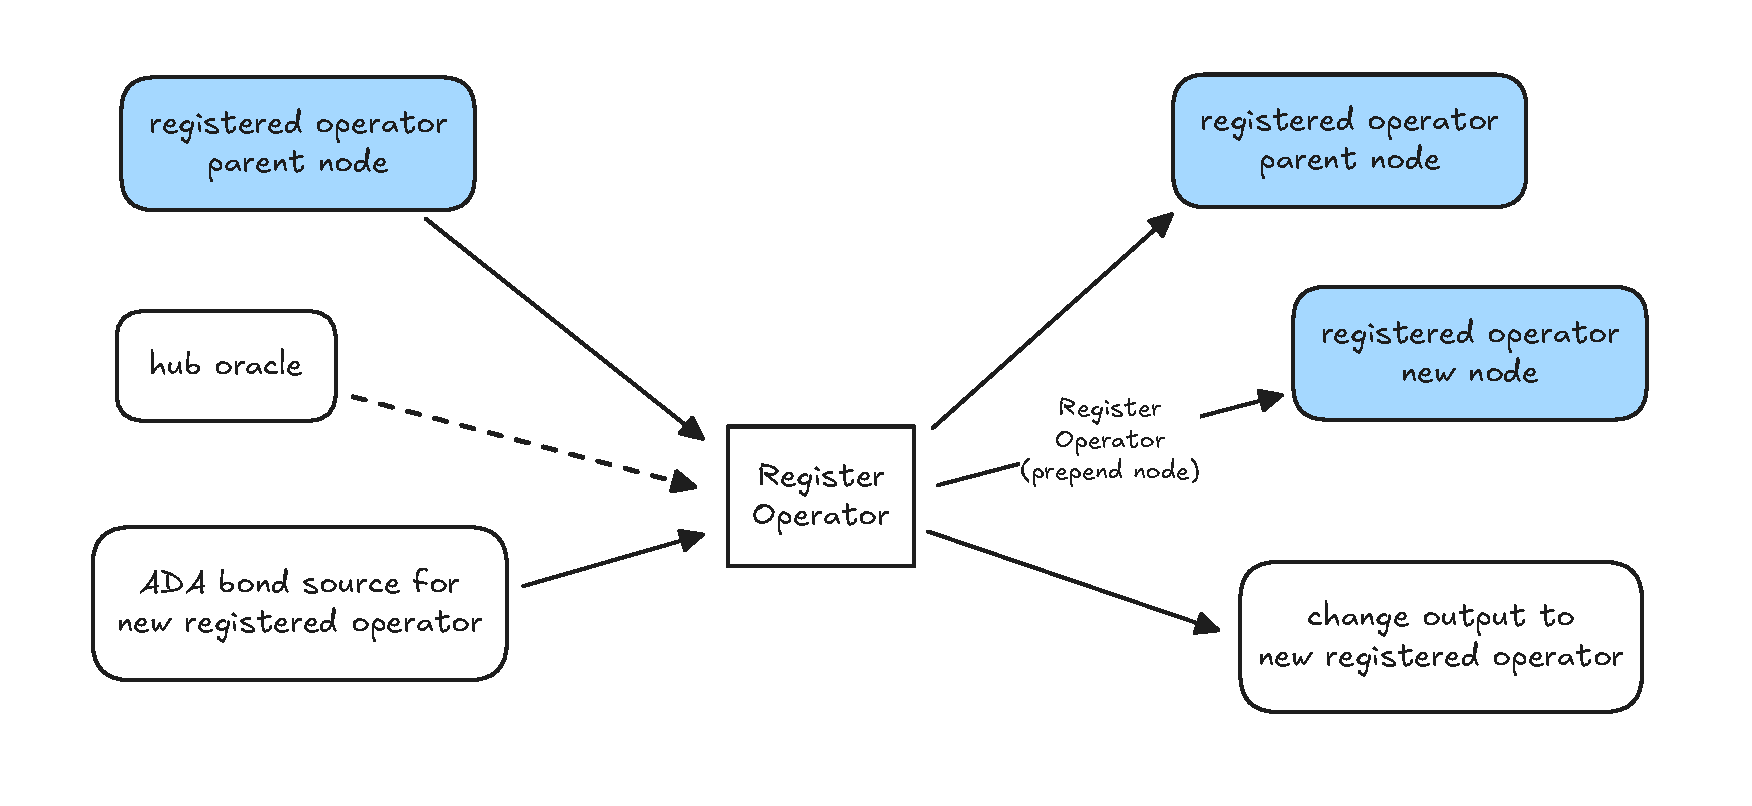
\includegraphics[width=\txDiagramScale\linewidth]{\subfix{../images/tx-diagram/1-register-operator.pdf}}
\end{center}
\caption[Register operator]{Register an operator.}
\label{fig:tx-register-operator}
\end{figure}

[TODO]

\begin{figure}[htb]
\begin{center}
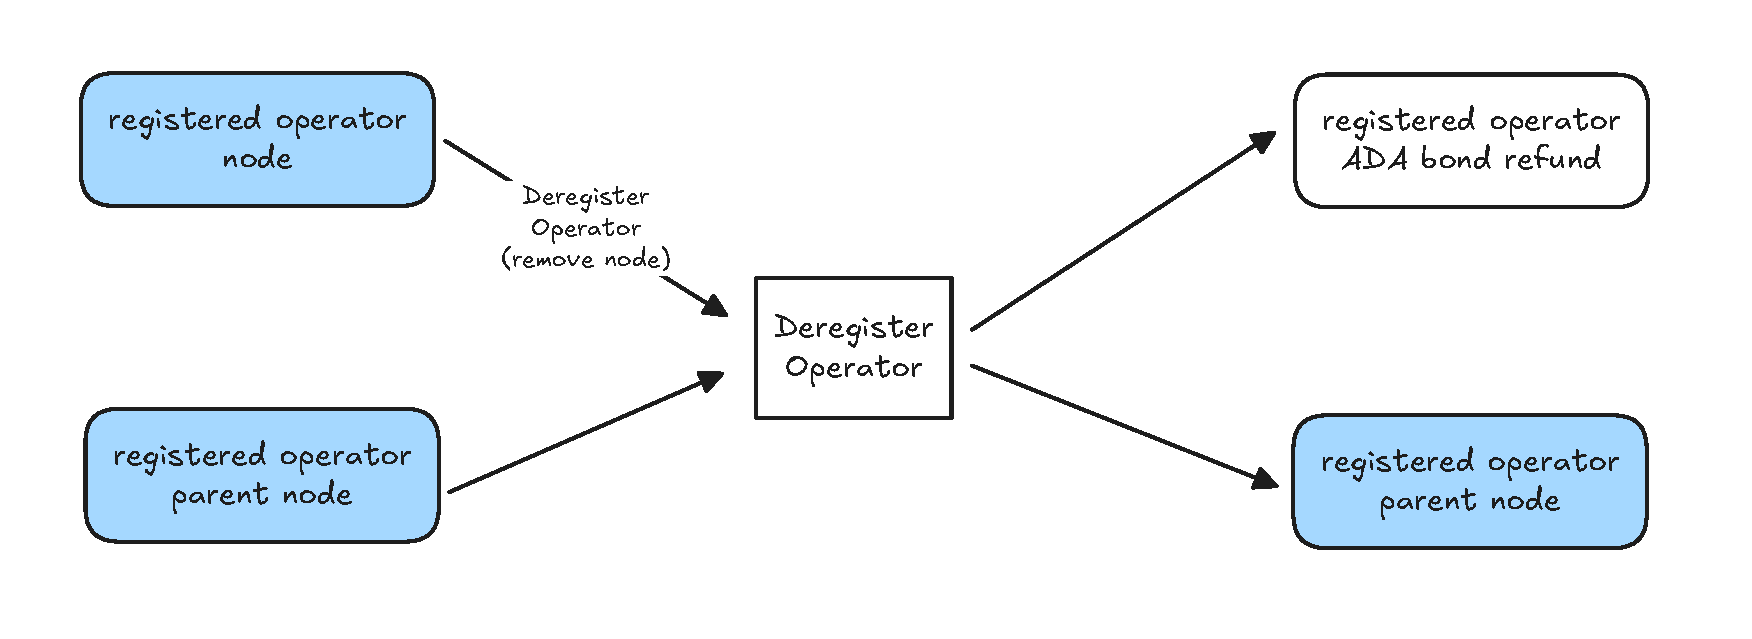
\includegraphics[width=\txDiagramScale\linewidth]{\subfix{../images/tx-diagram/2-deregister-operator.pdf}}
\end{center}
\caption[De-register operator]{De-register an operator.}
\label{fig:tx-deregister-operator}
\end{figure}

[TODO]

\begin{figure}[htb]
\begin{center}
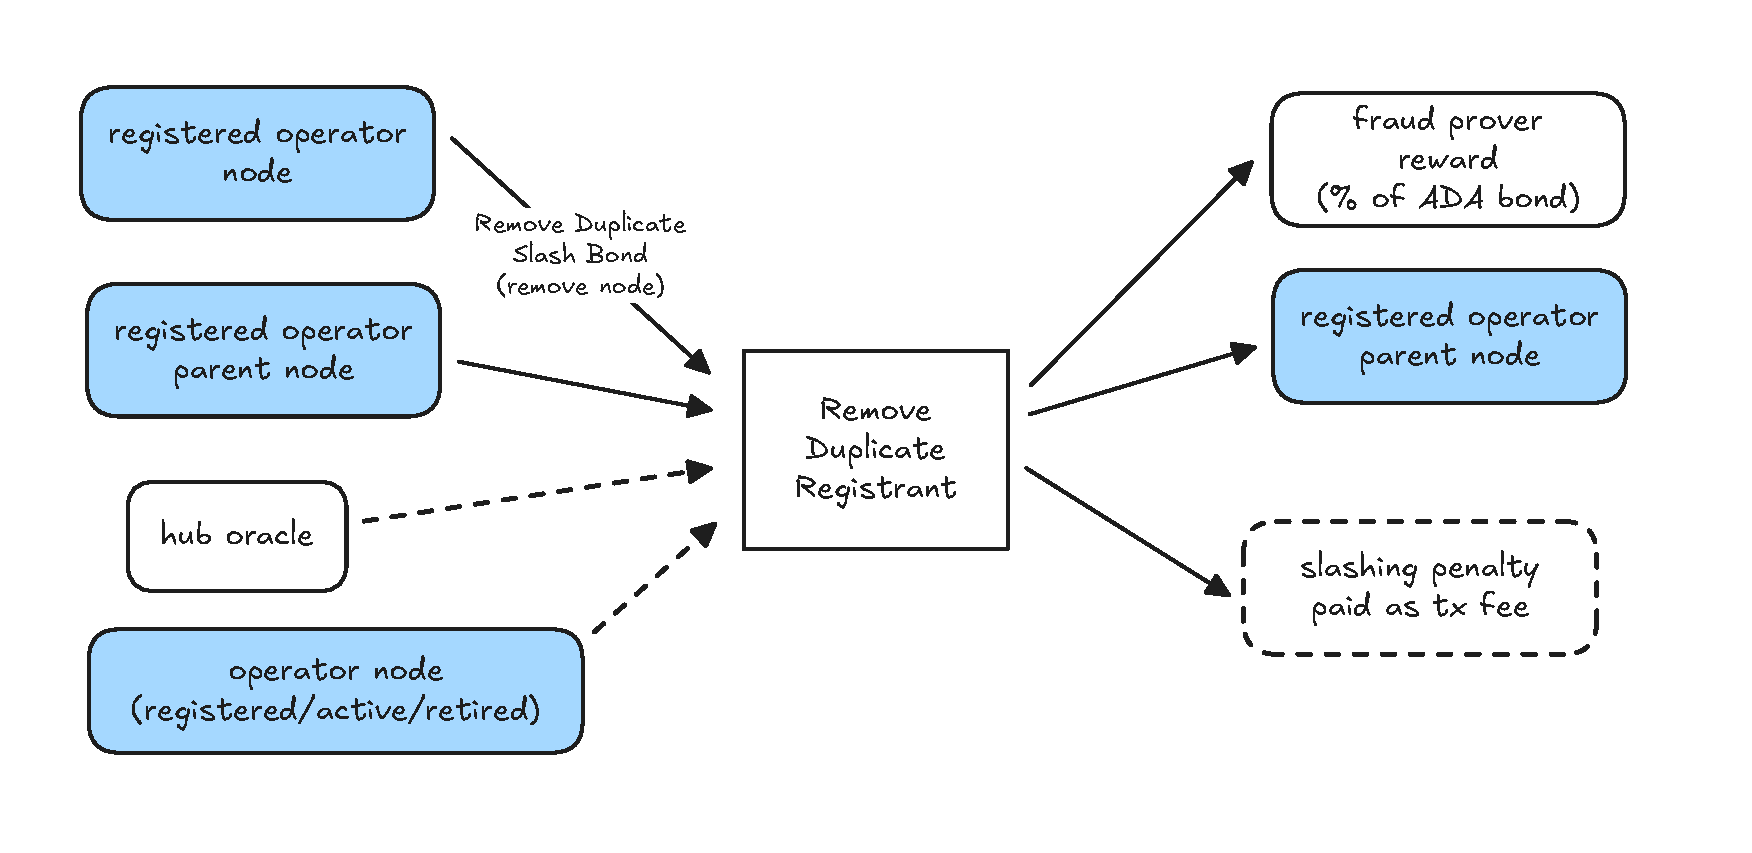
\includegraphics[width=\txDiagramScale\linewidth]{\subfix{../images/tx-diagram/3-remove-duplicate-registrant.pdf}}
\end{center}
\caption[Remove duplicate registrant]{Remove and slash a duplicate registered operator.}
\label{fig:tx-remove-duplicate-registrant}
\end{figure}

[TODO]

\begin{figure}[htb]
\begin{center}
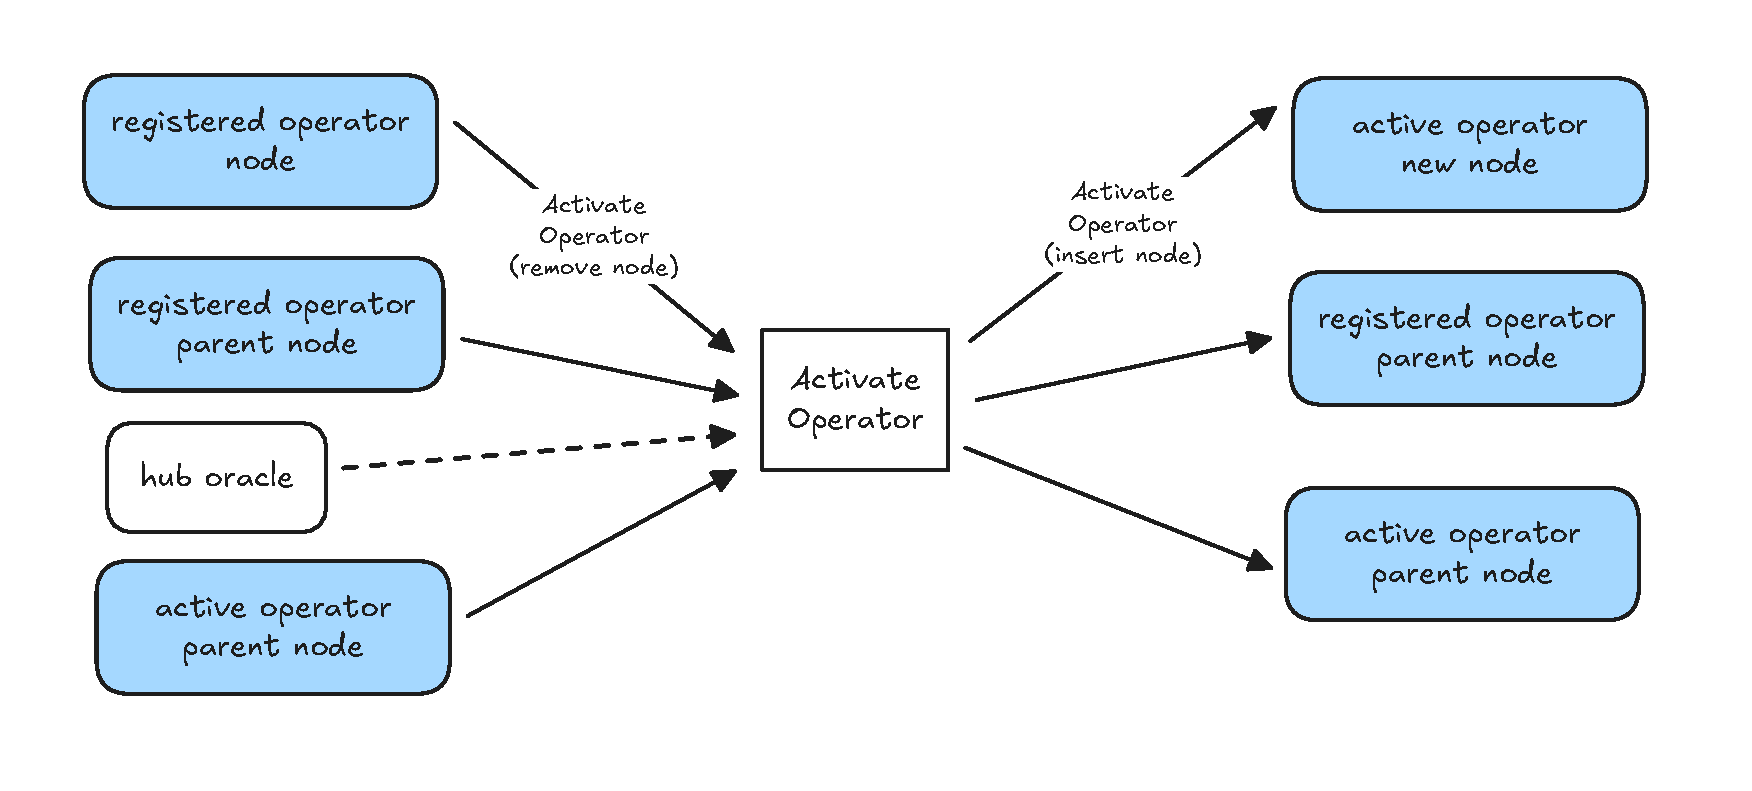
\includegraphics[width=\txDiagramScale\linewidth]{\subfix{../images/tx-diagram/4-activate-operator.pdf}}
\end{center}
\caption[Activate operator]{Activate a registered operator.}
\label{fig:tx-activate-operator}
\end{figure}

[TODO]

\begin{figure}[htb]
\begin{center}
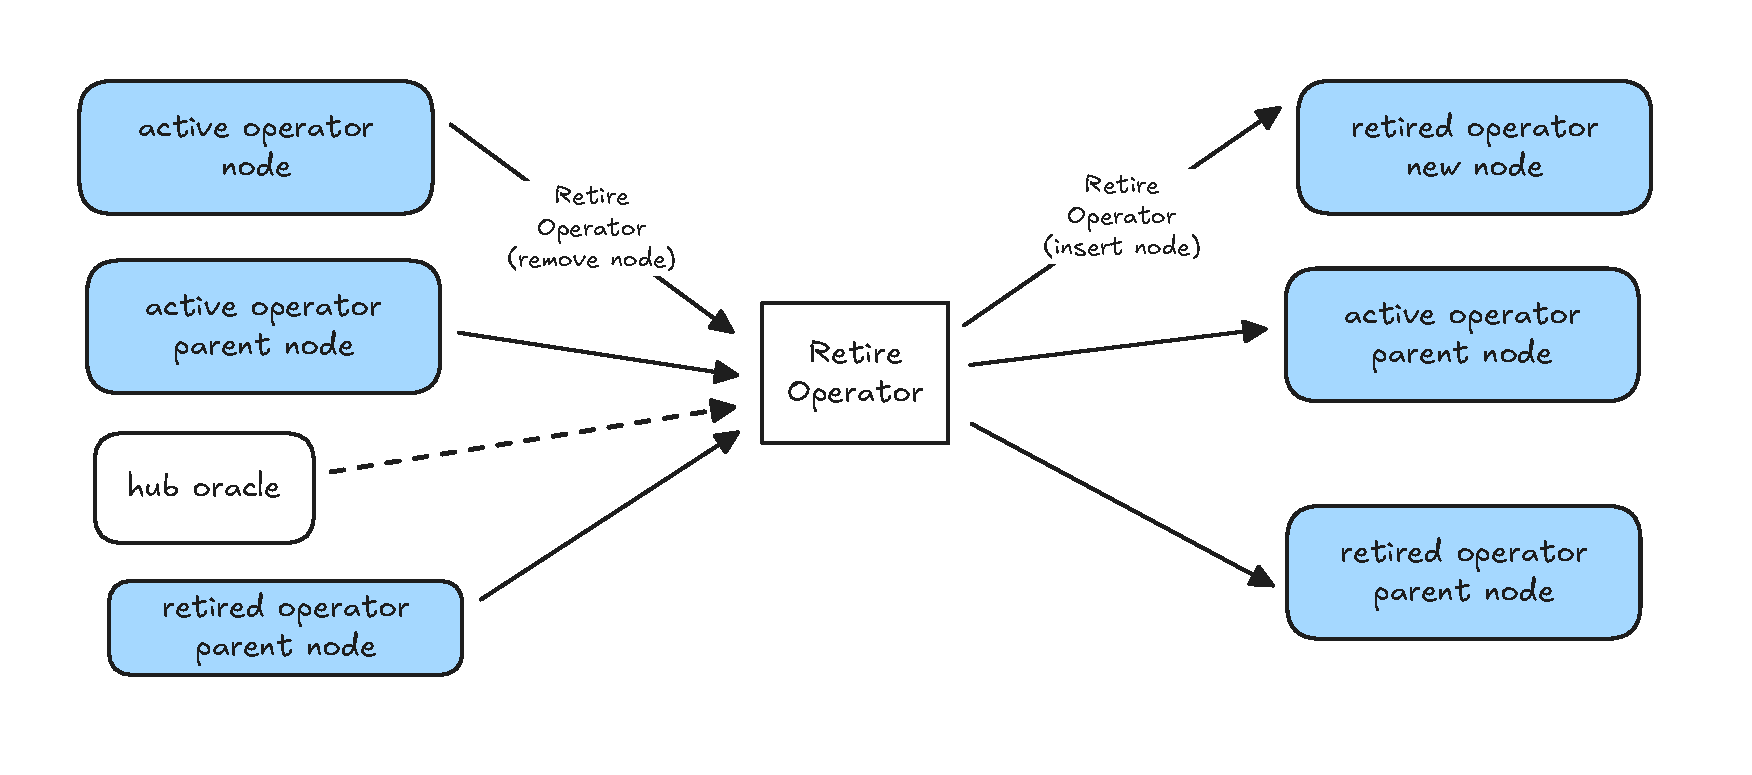
\includegraphics[width=\txDiagramScale\linewidth]{\subfix{../images/tx-diagram/5-retire-operator.pdf}}
\end{center}
\caption[Retire operator]{Retire an active operator.}
\label{fig:tx-retire-operator}
\end{figure}

[TODO]

\begin{figure}[htb]
\begin{center}
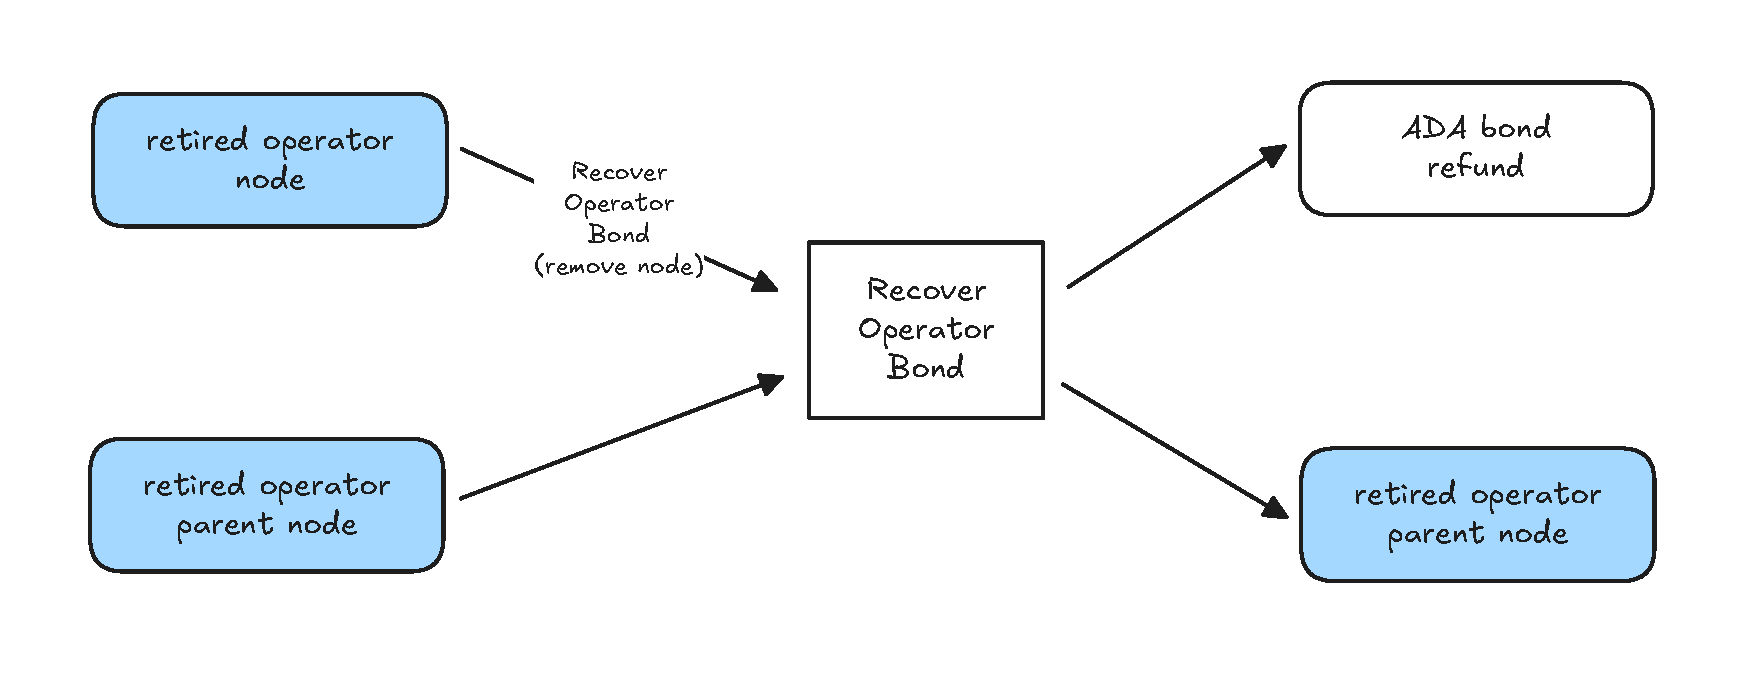
\includegraphics[width=\txDiagramScale\linewidth]{\subfix{../images/tx-diagram/6-recover-bond.pdf}}
\end{center}
\caption[Recover operator bond]{Recover a retired operator's bond.}
\label{fig:tx-recover-bond}
\end{figure}

[TODO]

\section{Scheduler}%
\label{h:midgard-l1-tx-scheduler}%

\begin{figure}[htb]
\begin{center}
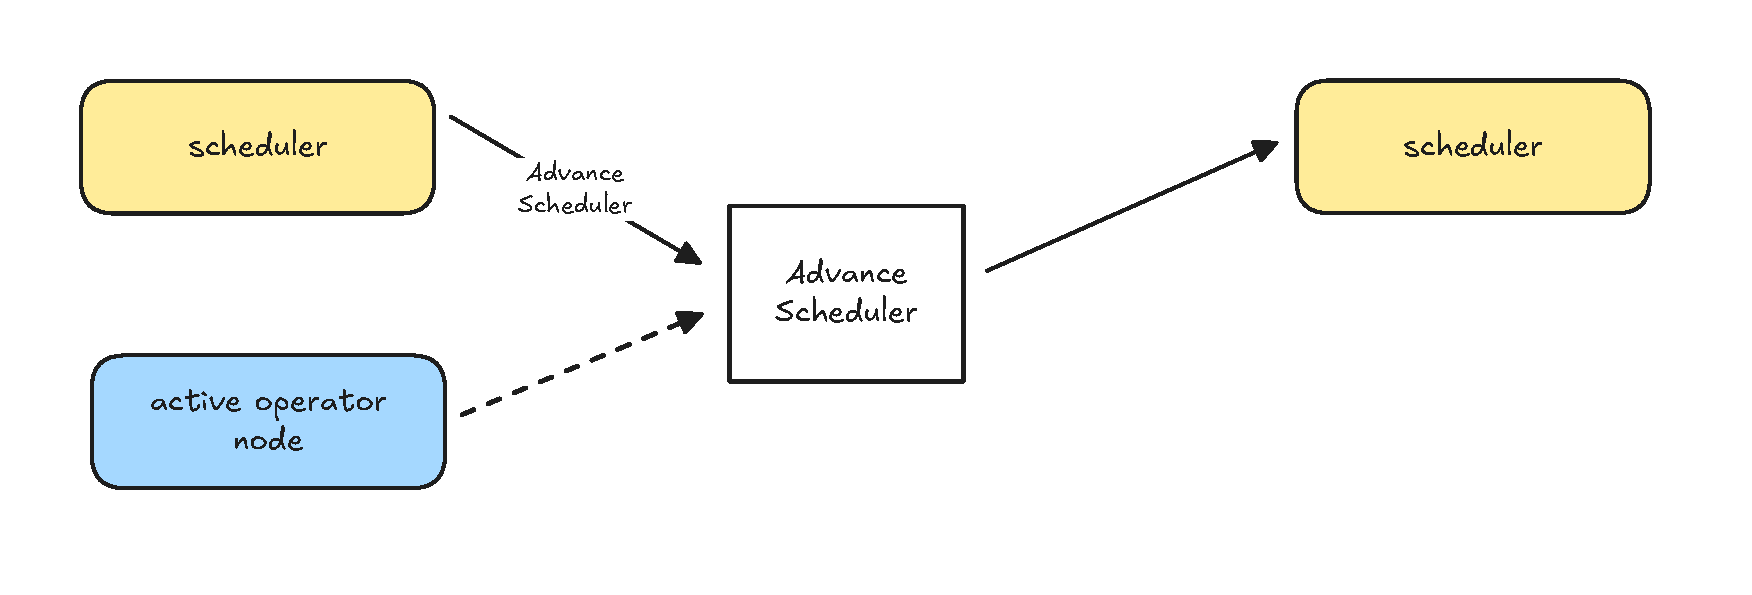
\includegraphics[width=\txDiagramScale\linewidth]{\subfix{../images/tx-diagram/7-advance-scheduler.pdf}}
\end{center}
\caption[Advance scheduler]{Advance the scheduler to the next operator.}
\label{fig:tx-advance-operator}
\end{figure}

[TODO]

\begin{figure}[htb]
\begin{center}
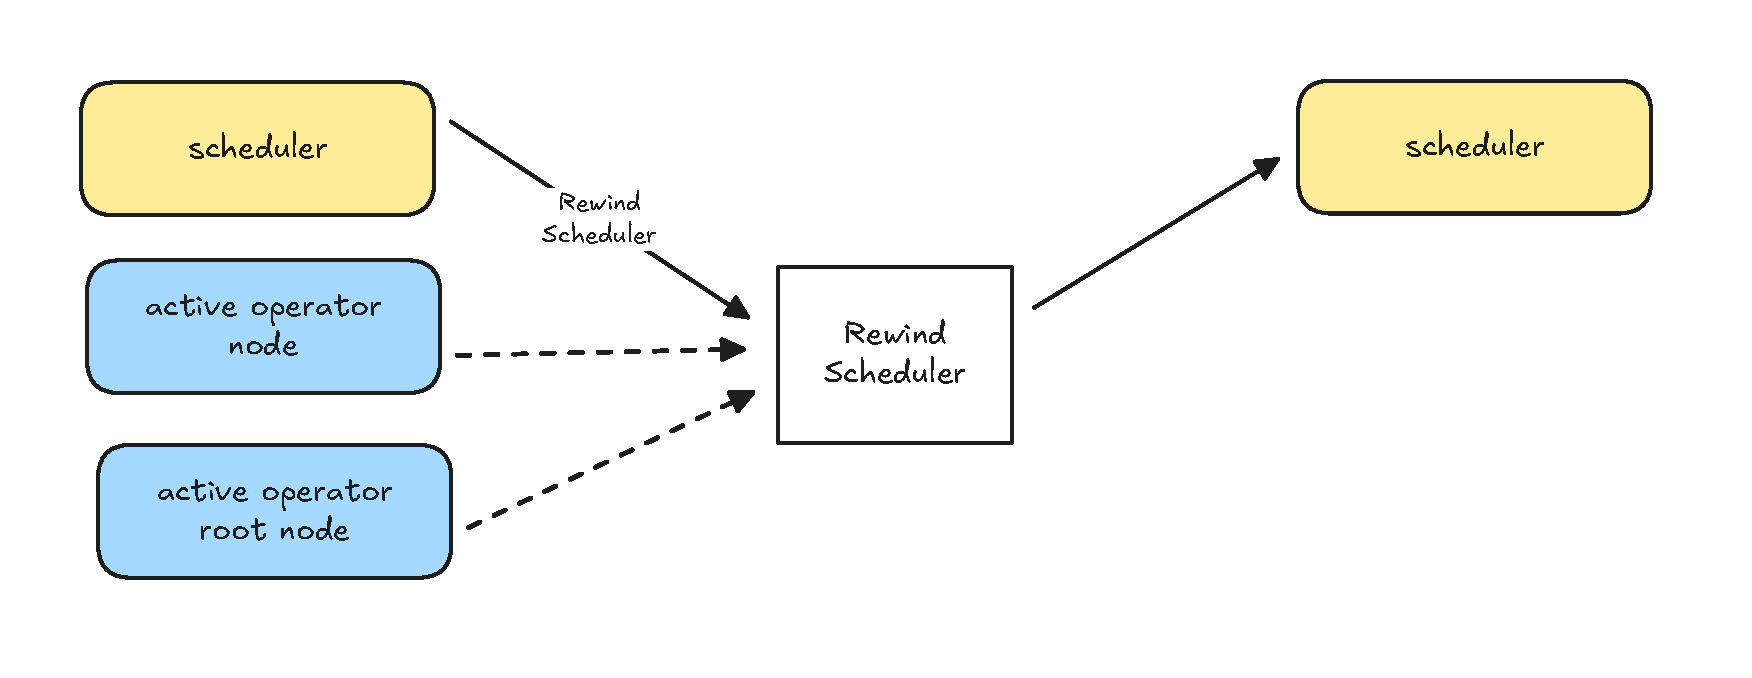
\includegraphics[width=\txDiagramScale\linewidth]{\subfix{../images/tx-diagram/8-rewind-scheduler.pdf}}
\end{center}
\caption[Rewind scheduler]{Rewind the scheduler to the first operator.}
\label{fig:tx-rewind-scheduler}
\end{figure}

[TODO]

\section{State queue}%
\label{h:midgard-l1-tx-state-queue}%

\begin{figure}[htb]
\begin{center}
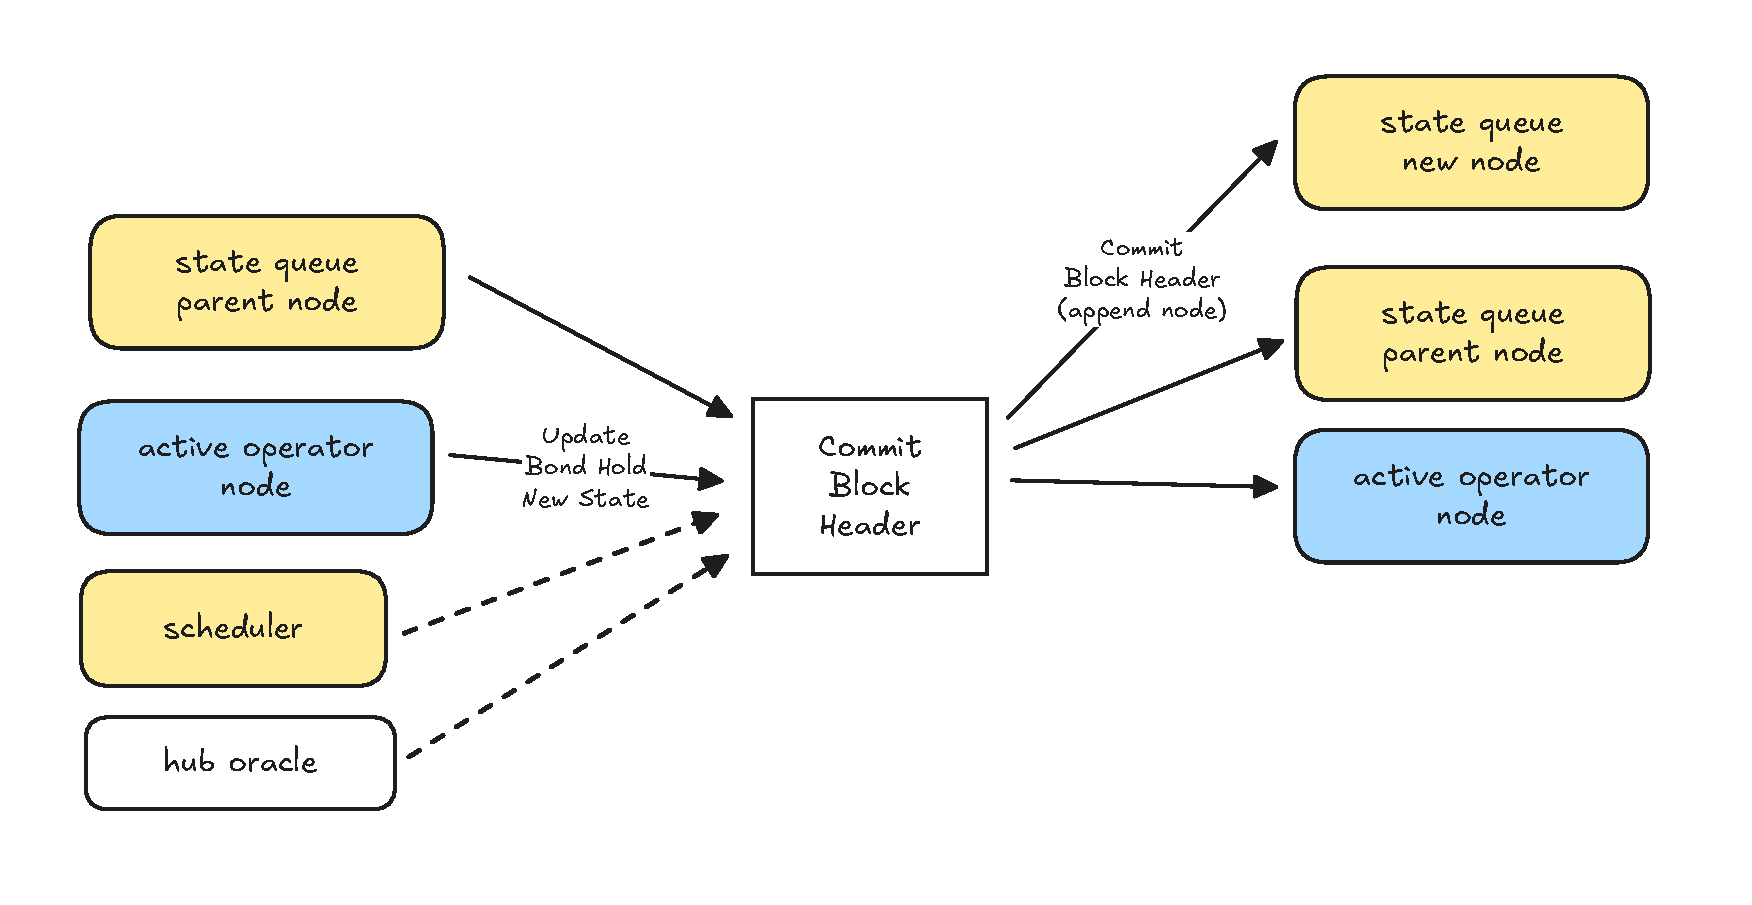
\includegraphics[width=\txDiagramScale\linewidth]{\subfix{../images/tx-diagram/9-commit-block-header.pdf}}
\end{center}
\caption[Commit block header]{Commit a block header to the state queue.}
\label{fig:tx-commit-block-header}
\end{figure}

[TODO]

\begin{figure}[htb]
\begin{center}
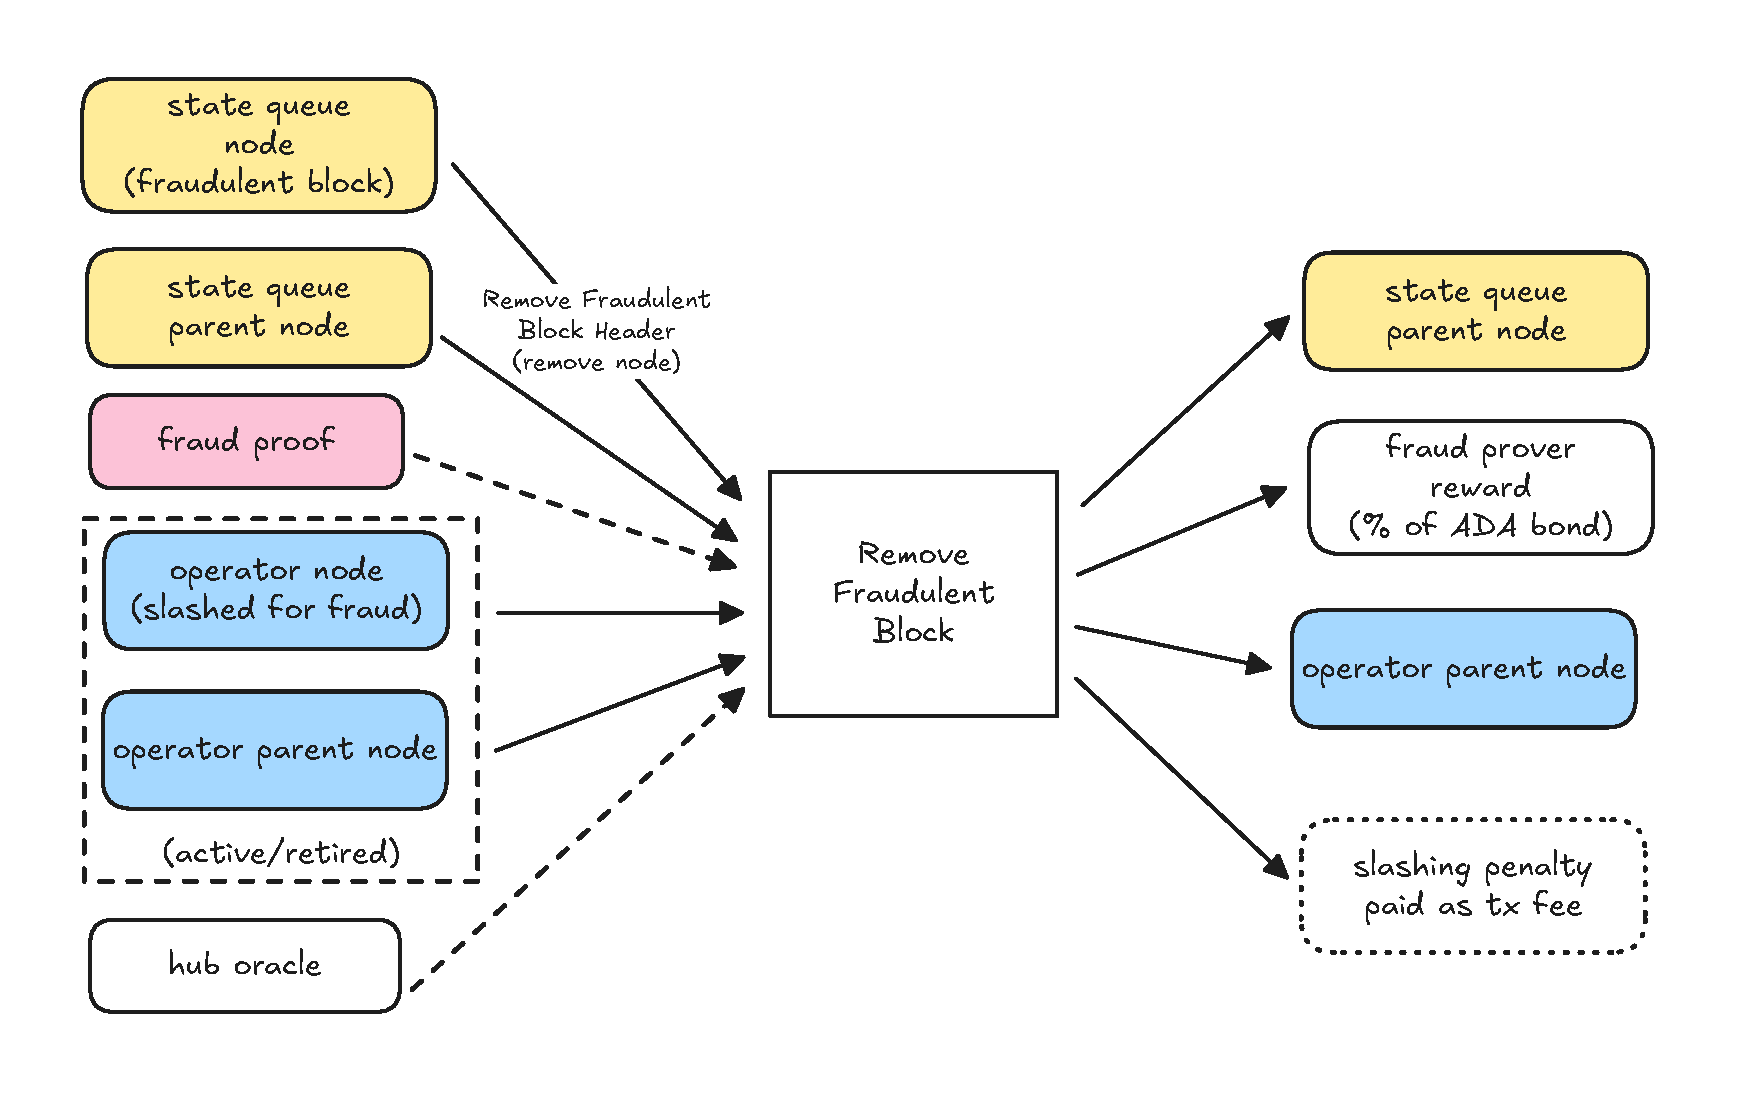
\includegraphics[width=\txDiagramScale\linewidth]{\subfix{../images/tx-diagram/A-remove-fraudulent-block-header.pdf}}
\end{center}
\caption[Remove fraudulent block header]{Remove a fraudulent block header and slash its operator.}
\label{fig:tx-remove-fraudulent-block-header}
\end{figure}

[TODO]

\begin{figure}[htb]
\begin{center}
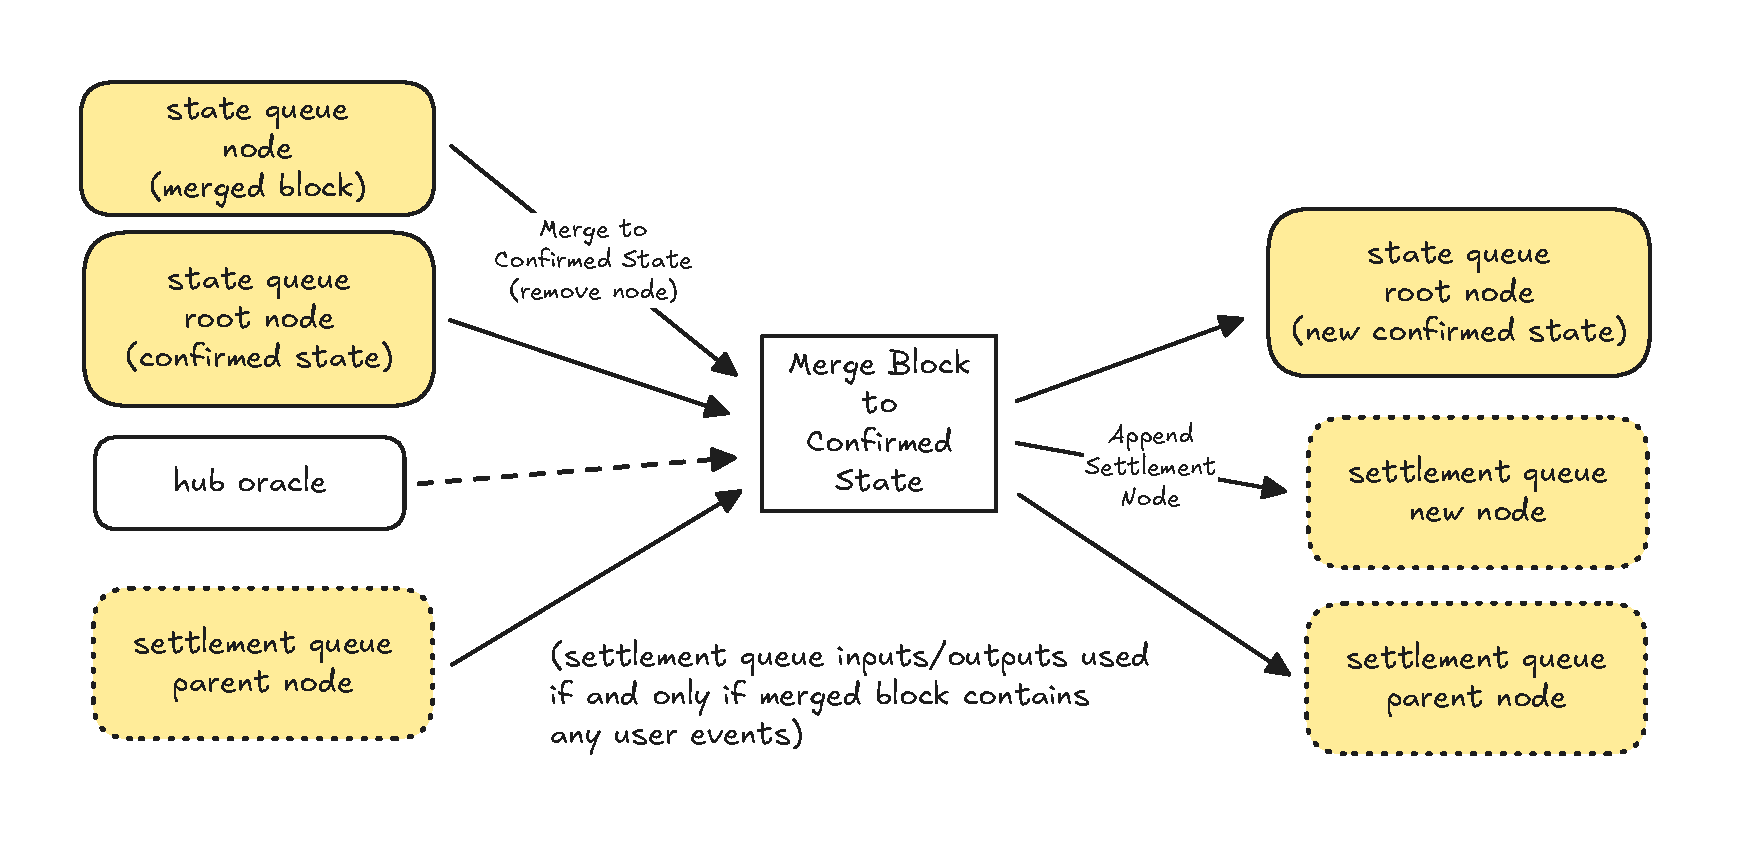
\includegraphics[width=\txDiagramScale\linewidth]{\subfix{../images/tx-diagram/B-merge-to-confirmed-state.pdf}}
\end{center}
\caption[Merge to confirmed state]{Merge a mature block header to the confirmed state.}
\label{fig:tx-merge-to-confirmed-state}
\end{figure}

[TODO]

\section{User events}%
\label{h:midgard-l1-tx-user-events}%

\begin{figure}[htb]
\begin{center}
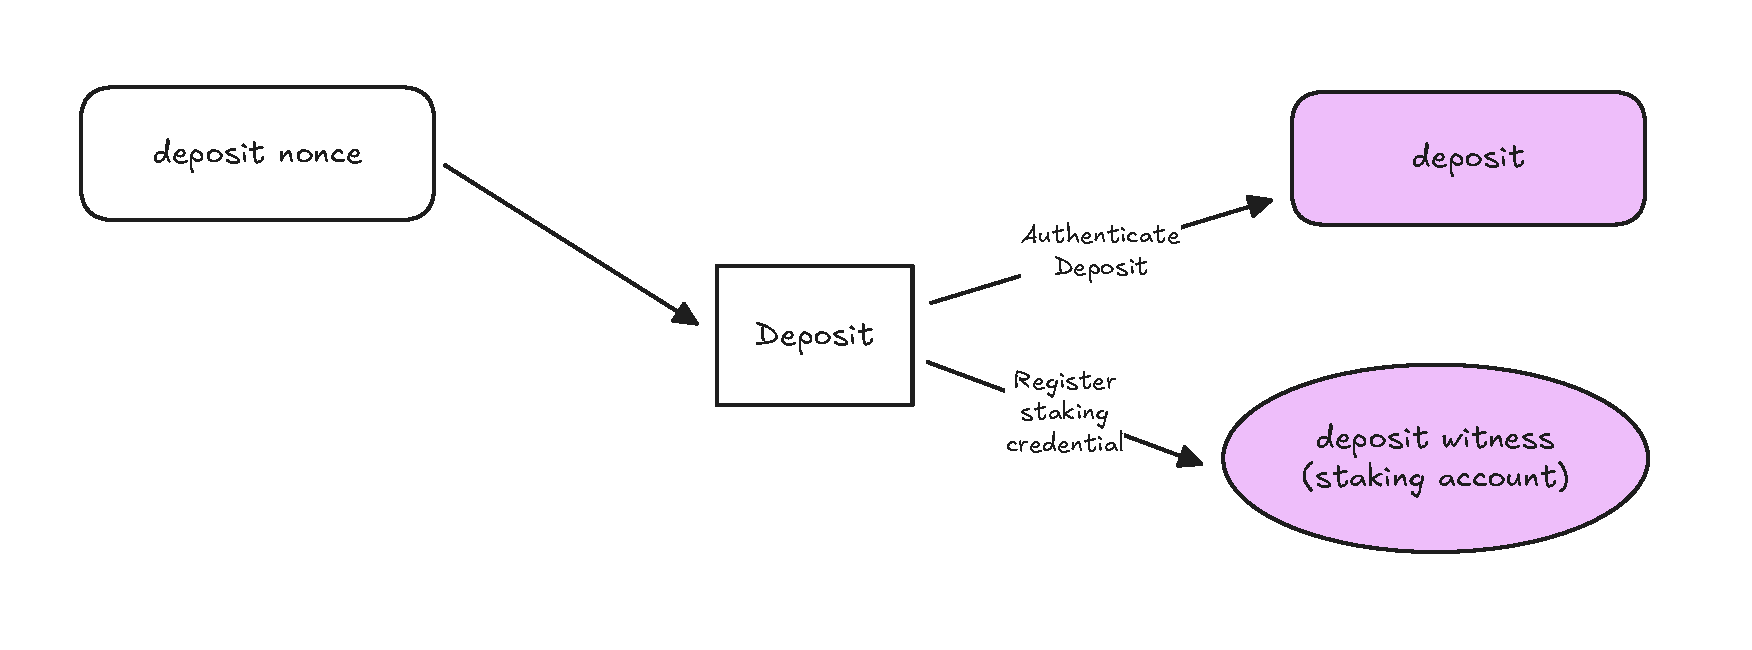
\includegraphics[width=\txDiagramScale\linewidth]{\subfix{../images/tx-diagram/C-deposit.pdf}}
\end{center}
\caption[Create deposit]{Create an L1 deposit for Midgard.}
\label{fig:tx-deposit}
\end{figure}

[TODO]

\begin{figure}[htb]
\begin{center}
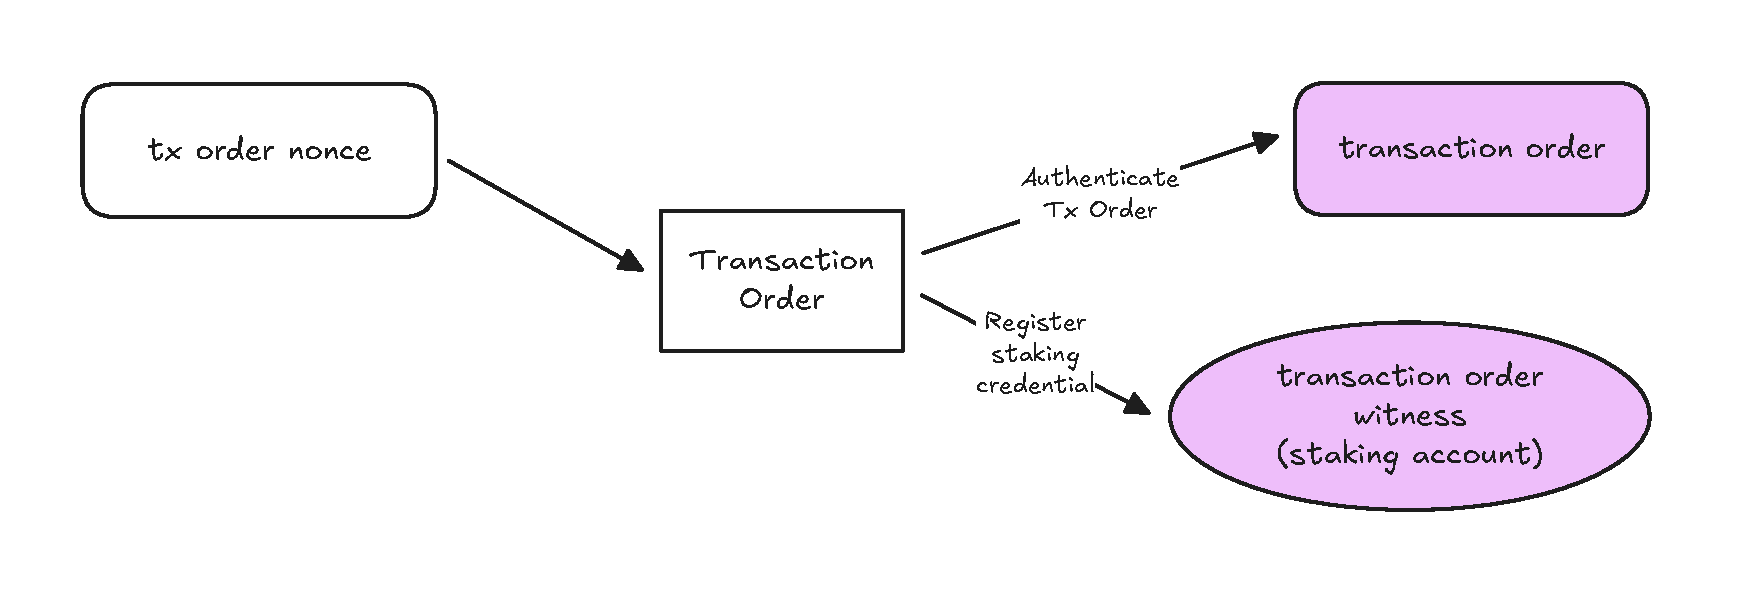
\includegraphics[width=\txDiagramScale\linewidth]{\subfix{../images/tx-diagram/D-tx-order.pdf}}
\end{center}
\caption[Create tx order]{Create a transaction order for Midgard.}
\label{fig:tx-transaction-order}
\end{figure}

[TODO]

\begin{figure}[htb]
\begin{center}
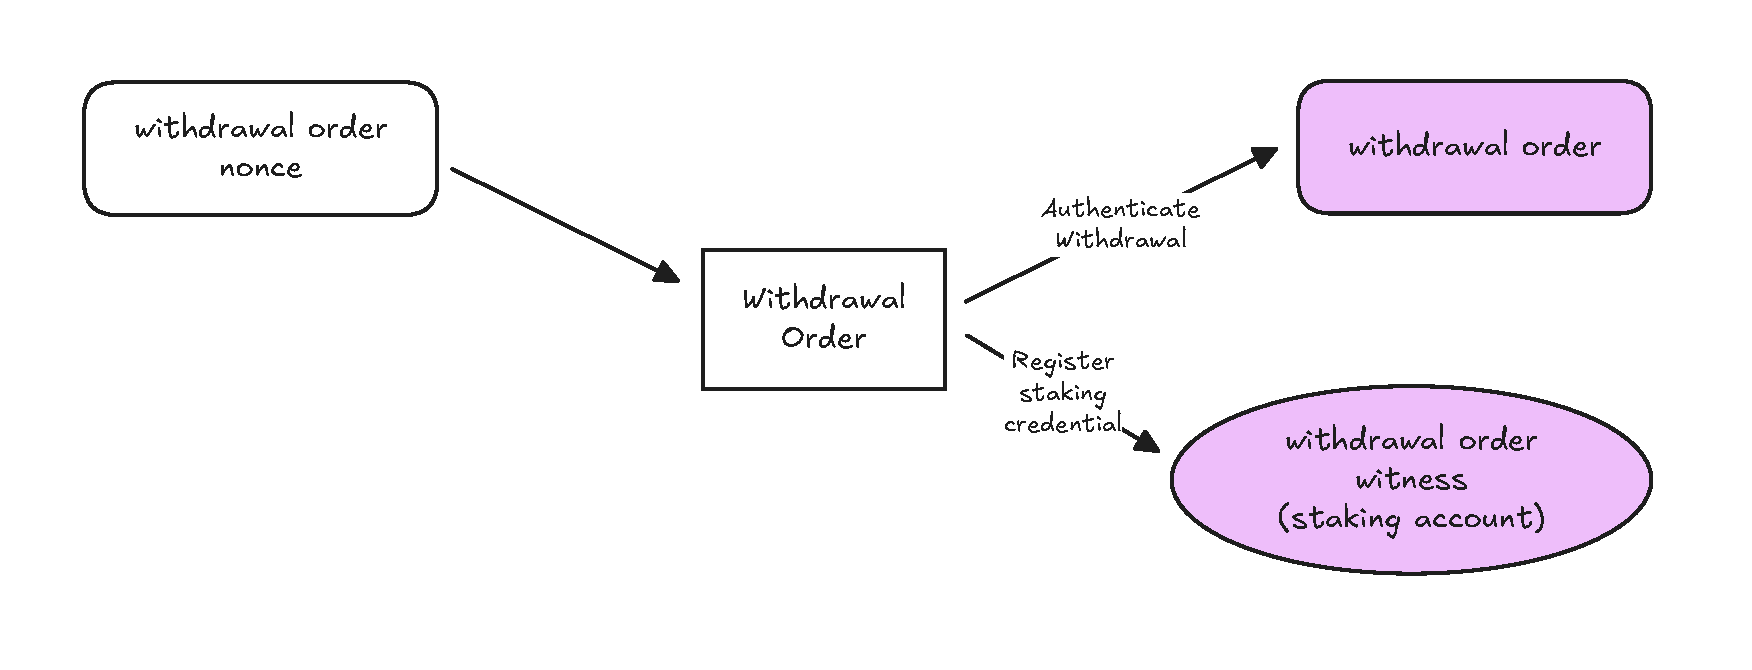
\includegraphics[width=\txDiagramScale\linewidth]{\subfix{../images/tx-diagram/E-withdrawal-order.pdf}}
\end{center}
\caption[Create withdrawal order]{Create a withdrawal order for Midgard.}
\label{fig:tx-withdrawal-order}
\end{figure}

[TODO]

\section{Settlement queue}%
\label{h:midgard-l1-tx-settlement-queue}%

\begin{figure}[htb]
\begin{center}
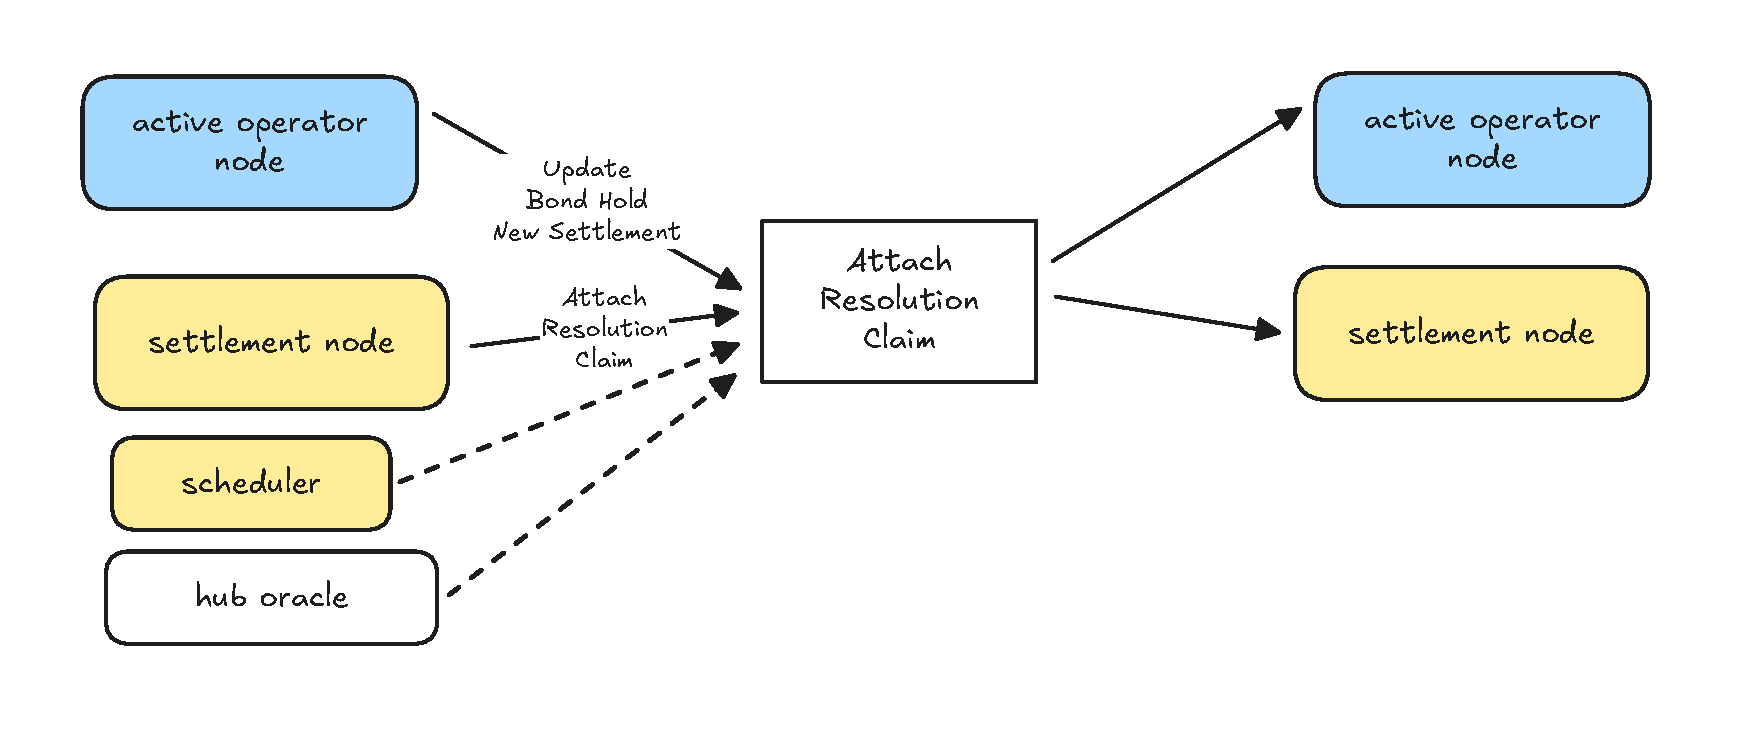
\includegraphics[width=\txDiagramScale\linewidth]{\subfix{../images/tx-diagram/F-attach-resolution-claim.pdf}}
\end{center}
\caption[Attach resolution claim]{Attach an optimistic resolution claim to a settlement node.}
\label{fig:tx-attach-resolution-claim}
\end{figure}

[TODO]

\begin{figure}[htb]
\begin{center}
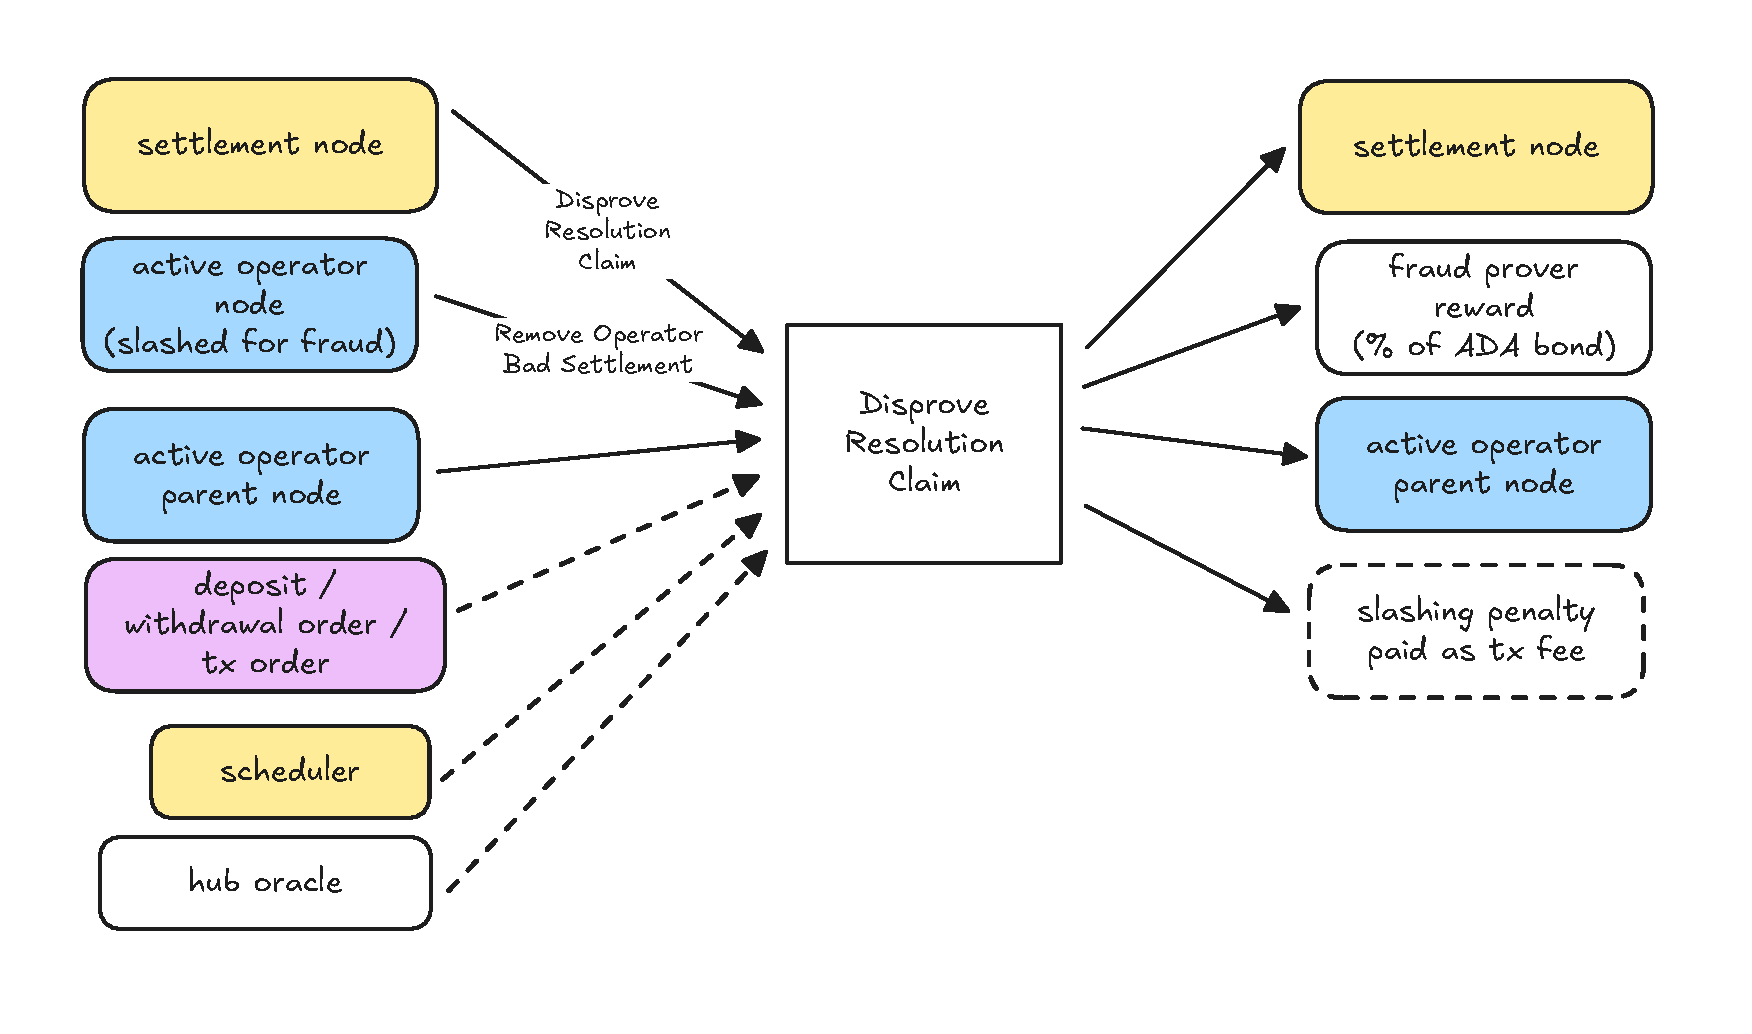
\includegraphics[width=\txDiagramScale\linewidth]{\subfix{../images/tx-diagram/G-disprove-resolution-claim.pdf}}
\end{center}
\caption[Disprove resolution claim]{Disprove an optimistic resolution claim of a settlement node.}
\label{fig:tx-disprove-resolution-claim}
\end{figure}

[TODO]

\begin{figure}[htb]
\begin{center}
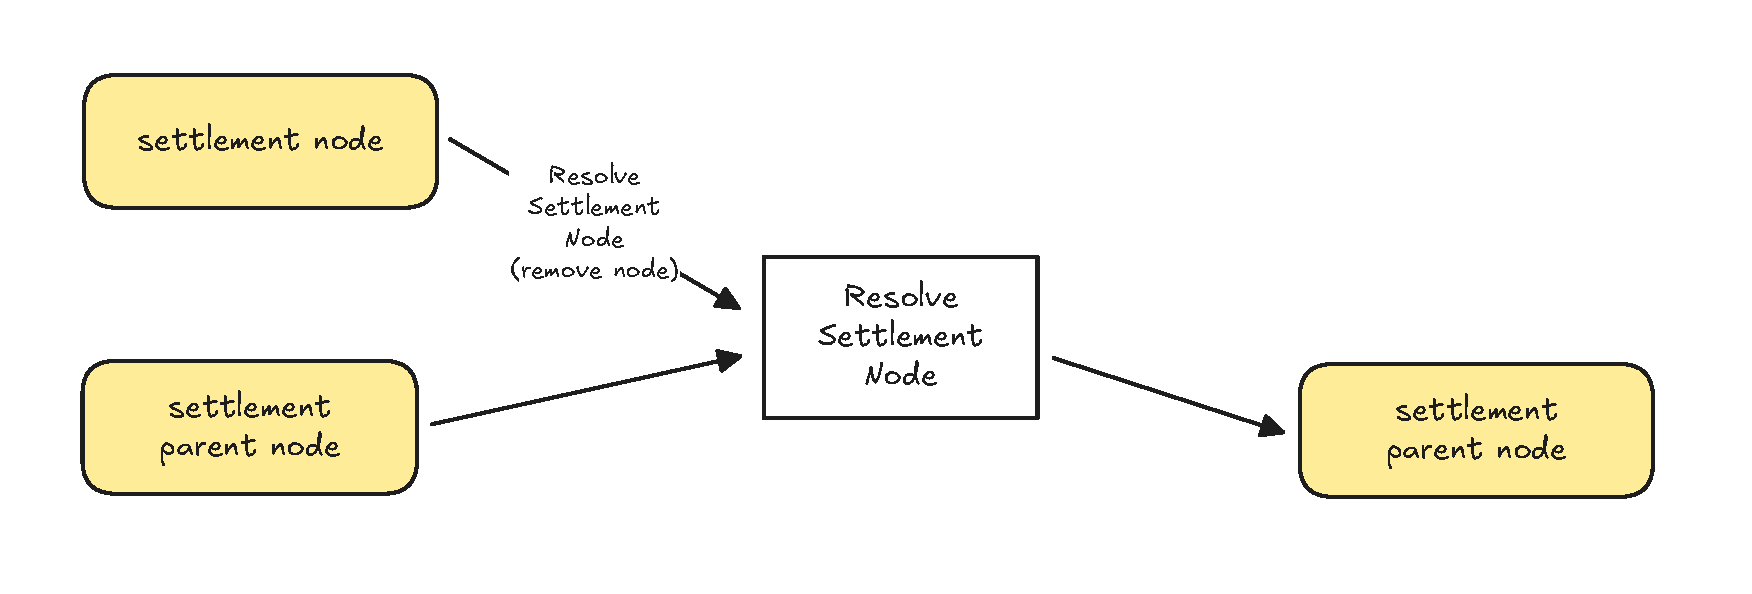
\includegraphics[width=\txDiagramScale\linewidth]{\subfix{../images/tx-diagram/H-resolve-settlement-node.pdf}}
\end{center}
\caption[Resolve settlement node]{Resolve a settlement node after its resolution claim matures.}
\label{fig:tx-resolve-settlement-node}
\end{figure}

[TODO]

\section{Fraud proofs}%
\label{h:midgard-l1-tx-fraud-proofs}%

\begin{figure}[htb]
\begin{center}
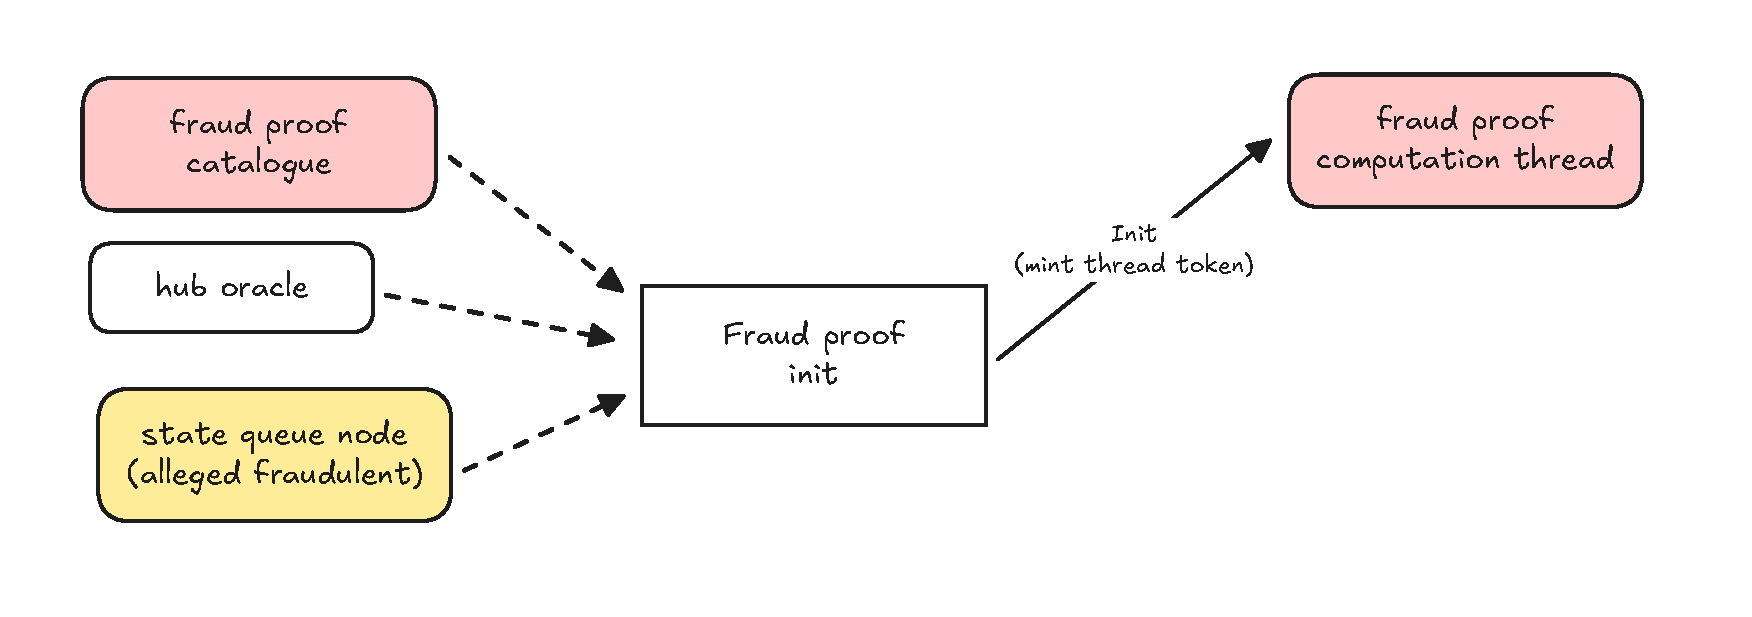
\includegraphics[width=\txDiagramScale\linewidth]{\subfix{../images/tx-diagram/I-fraud-proof-init.pdf}}
\end{center}
\caption[Fraud proof init]{Initialize the verification of a fraud proof.}
\label{fig:tx-fraud-proof-init}
\end{figure}

[TODO]

\begin{figure}[htb]
\begin{center}
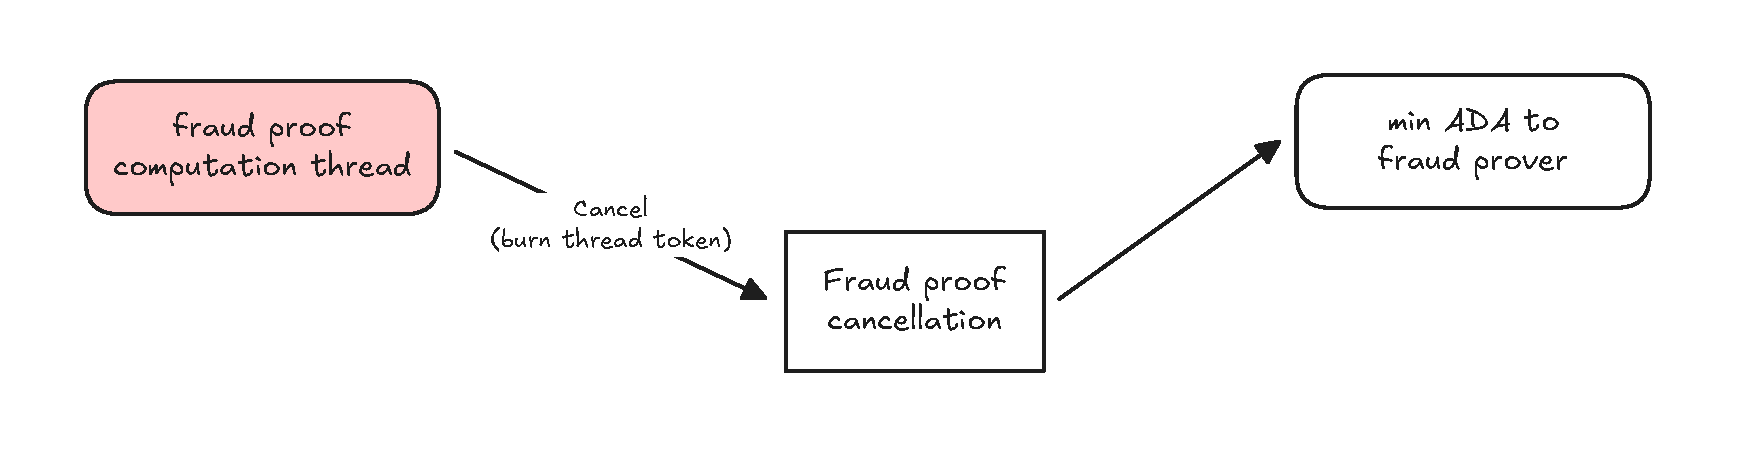
\includegraphics[width=\txDiagramScale\linewidth]{\subfix{../images/tx-diagram/J-fraud-proof-cancel.pdf}}
\end{center}
\caption[Fraud proof cancel]{Cancel the verification of a fraud proof.}
\label{fig:tx-fraud-proof-cancel}
\end{figure}

[TODO]

\begin{figure}[htb]
\begin{center}
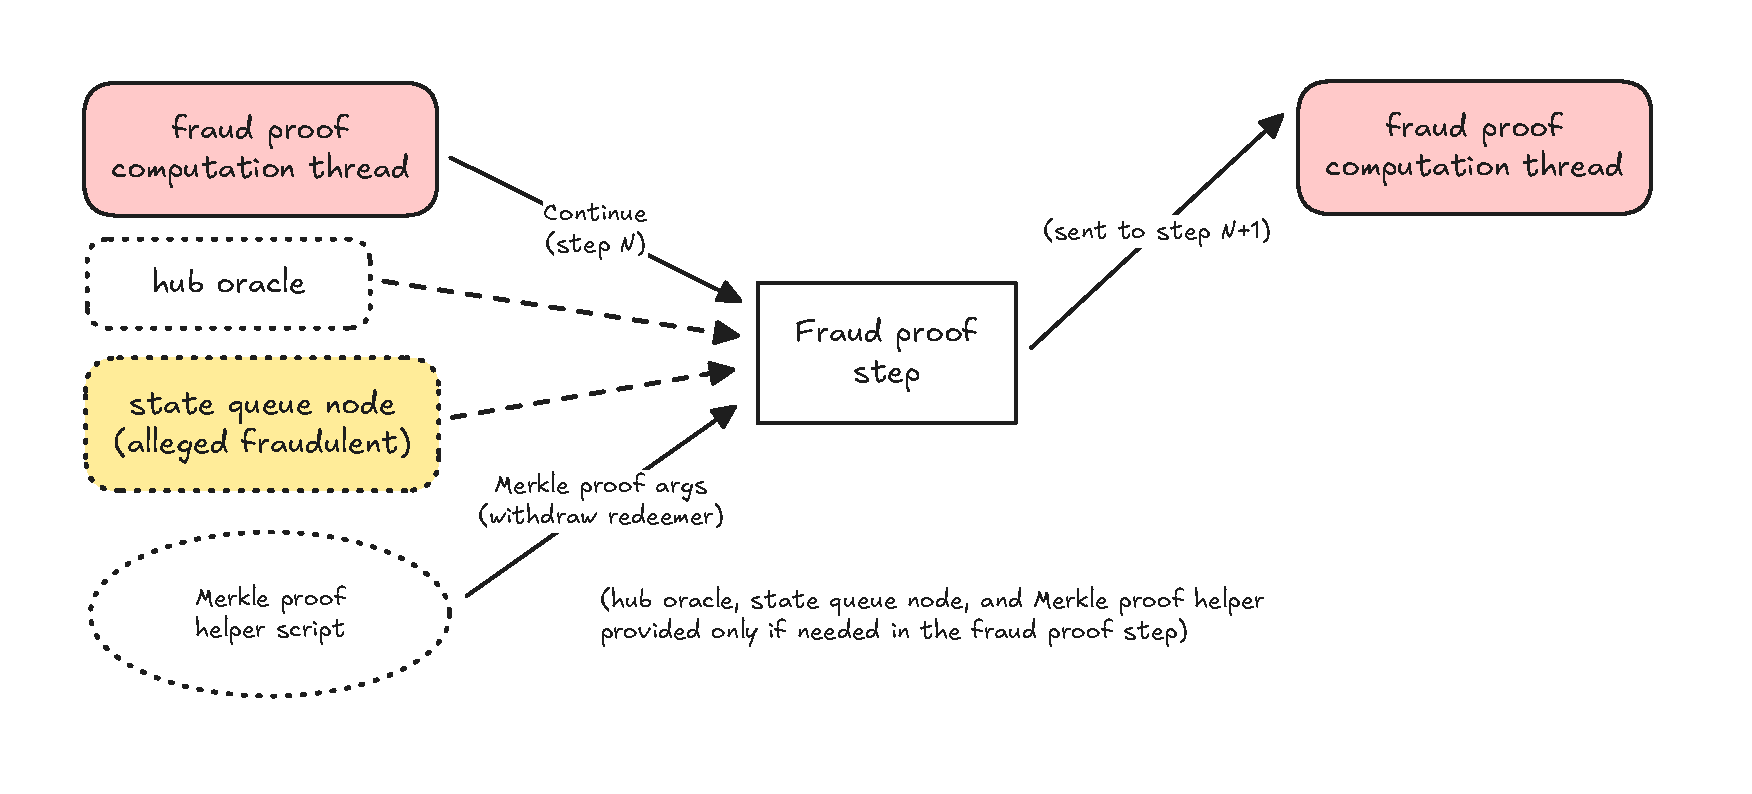
\includegraphics[width=\txDiagramScale\linewidth]{\subfix{../images/tx-diagram/K-fraud-proof-step.pdf}}
\end{center}
\caption[Fraud proof step]{Perform a verification step of a fraud proof.}
\label{fig:tx-fraud-proof-step}
\end{figure}

[TODO]

\begin{figure}[htb]
\begin{center}
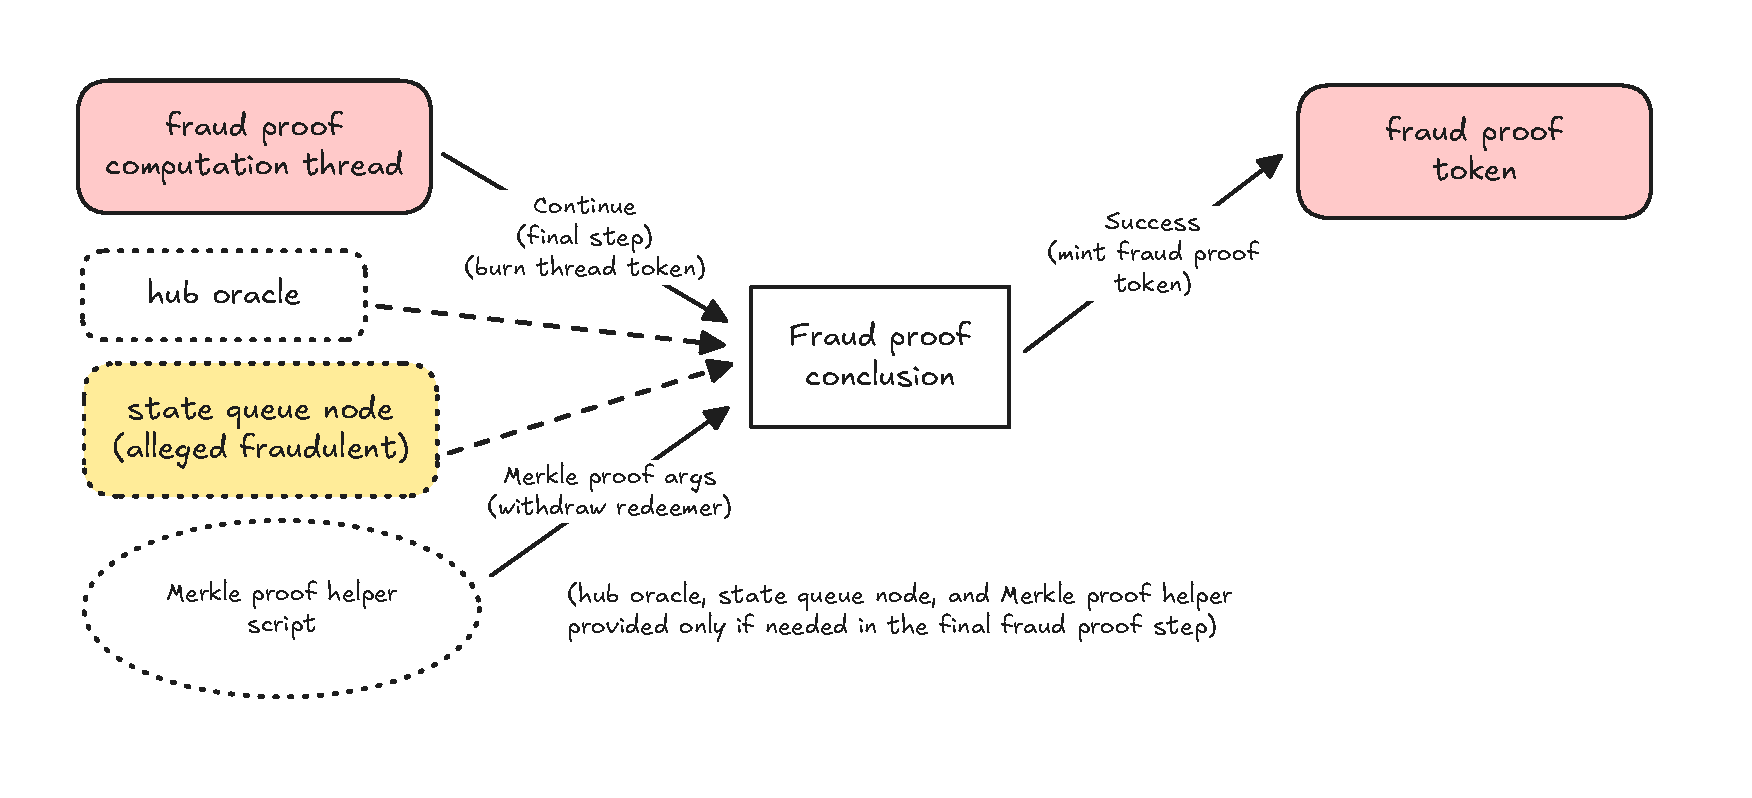
\includegraphics[width=\txDiagramScale\linewidth]{\subfix{../images/tx-diagram/L-fraud-proof-conclude.pdf}}
\end{center}
\caption[Fraud proof conclude]{Conclude the verification of a fraud proof by performing its final step.}
\label{fig:tx-fraud-proof-conclude}
\end{figure}

[TODO]

\end{document}
